%----------------------------------------------------------------------------
\chapter{Validáció}
\label{chp:validation}
%----------------------------------------------------------------------------

Ebben a fejezetben az alkalmazás működését teszteljük, majd több mérést végzünk különböző teljesítményparamétereket vizsgálva, az előbbit erre kialakított tesztkörnyezetben, az utóbbit már annak a labornak a gépein, ahol várhatóan éles használatban lesz.

%----------------------------------------------------------------------------
\section{Tesztelés}
%----------------------------------------------------------------------------

%
\subsection{Tesztkörnyezet és a program bemenete}
%

A tesztelést a program fejlesztésére használt gépen végeztem el, a terítésben résztvevő gépek Vagrant-tal létrehozott, VirtualBox által futtatott virtuális gépek, amelyeken az operációs rendszer 32-bites 12.04 verziójú Ubuntu\cite{ubuntu}. A virtuális gépekre csak a legszükségesebb szoftverek lettek telepítve, egymással és a gazdagéppel egy közös privát hálózaton voltak. A program futtatásához megadott labormodell fontosabb paraméterei:

\begin{itemize}
  \item Két különböző virtuális gép van benne: egy ``sima'' VirtualMachine típusú ``customvm\_test'' nevű és egy Vagrant\_VM típusú ``vagrantvm\_test'' nevű
  \item 6 db. Computer, amik közül az egyik dedikált seed (labpc101-105, seed)
  \item A terítés célállapotát reprezentáló ``mixed\_test'' nevű Lab, ami mindegyik gépre mindkét virtuális gép terítését írja elő
  \item Labpc105-re nem fér el egyik VM sem, 104-nek nincs elég memóriája szintén egyikhez sem, 103 architektúrája nem kompatibilis a Vagrant\_VM típusú virtuális géppel, 102-re már telepítve van ``customvm\_test''. Labpc101-re mindkettő terülhet
\end{itemize}

A futtatáshoz a ``mixed\_test'' nevű célállapotot adtam meg, mint értelemszerűen az egyetlen felvett ilyet.

%
\subsection{Program futásának végigkövetése}
%

Mielőtt végigkövetnénk a futtatást érdemes végiggondolni, hogy mi lenne az elvárt eredmény a fent ismertetett bemenet függvényében, milyen fontosabb lépéseket és milyen sorrendben fog a program végrehajtani:

\begin{enumerate}
  \item Figyelmeztetés, hogy 105 és 104-re semelyik, 103 és 102-re pedig egyik VM nem fog terülni.
  \item ``vagrantvm\_test'' inicializálása Vagrant-tal, majd becsomagolása egy .zip archívumba
  \item Mindkét VM felmásolása a seed gépre, mindkettőhöz torrent fájl létrehozása
  \item Torrentkliens futtatása a seed gépen
  \item Torrent fájlok átmásolása a labpc101-103 gépekre
  \item Torrentkliens futtatása a labpc101-103 gépeken
  \item A letöltések sikeres befejezése után a modell frissítése
\end{enumerate}

A program indítása után rögtön a várt figyelmeztetések jelennek meg a konzolablakban:\\\\
\code{2015-12-08 00:21:48 WARNING hu.bme.mit.vmdistribution.app.EMFModelUtil isCompatible WARNING:\_Computer:labpc104 is not compatible with Virtual Machine:vagrantvm\_test, Not enough RAM!}\\
\code{2015-12-08 00:21:48 WARNING hu.bme.mit.vmdistribution.app.EMFModelUtil isCompatible WARNING:\_Computer:labpc104 is not compatible with Virtual Machine:customvm\_test, Not enough RAM!}\\
\code{2015-12-08 00:21:48 WARNING hu.bme.mit.vmdistribution.app.EMFModelUtil isCompatible WARNING:\_Computer:labpc103 is not compatible with Virtual Machine:vagrantvm\_test, Architecture mismatch!}\\
\code{2015-12-08 00:21:48 WARNING hu.bme.mit.vmdistribution.app.EMFModelUtil hasEnoughSpace WARNING:\_Computer:labpc105 does not have enough free space for the new VMs! Available: 2000.0 MB, Required: 15500.0 MB}\\\\
Majd meghívódik a Vagrant, hogy létrehozza a ``vagrantvm\_test''-et, az~\ref{fig:vboxcap}-es~ábrán látható, hogy a VirtualBox VM-eket tartalmazó mappájába már bele is került az új virtuális gép és meg is jelenik annak a felületén.

\begin{figure}[ht]
\centering
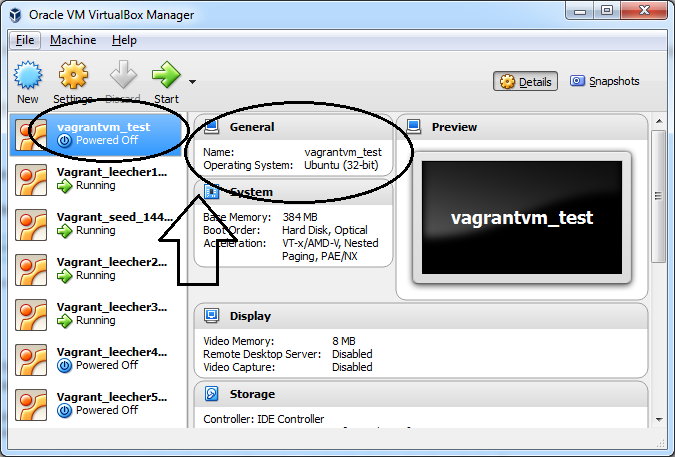
\includegraphics[width=100mm, keepaspectratio]{figures/test_vbox.png}
\caption{Vagrant által létrehozott virtuális gépek a VirtualBox-ban}
\label{fig:vboxcap}
\end{figure}
A kész virtuális gépből a program létrehoz egy tömörített .zip állományt\ldots\\\\
\code{2015-12-08 00:37:03 INFO hu.bme.mit.vmdistribution.app.vmutil.Archiver createZipArchive Creating Archive: E:\textbackslash{}vagrantvm\_test.zip}\\\\
\ldots majd a két VM felkerül a seed-re, ahogy az~\ref{fig:seed_files}-es~ábrán ez látszik is:  a seed-del SSH kapcsolat létesítése után kilistázzuk azoknak a mappáknak a tartalmát ahová a VM-eket tartalmazó zip fájlok, illetve az azok alapján készített torrent fájlok kerültek.

\begin{figure}[ht]
\centering
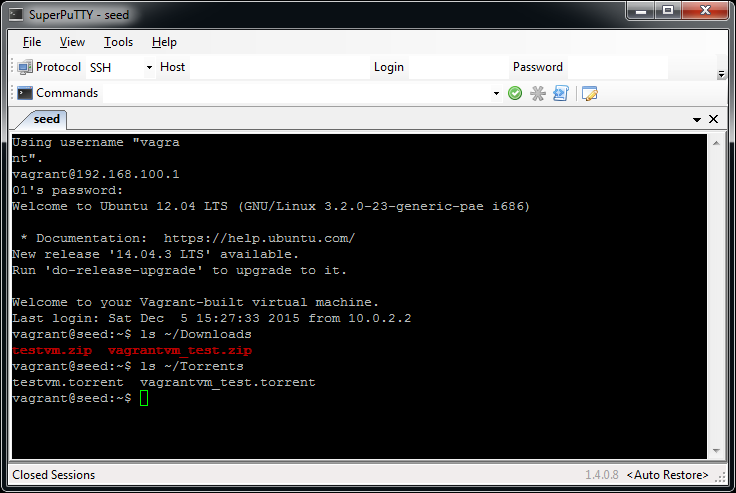
\includegraphics[width=120mm, keepaspectratio]{figures/test_seed_files.png}
\caption{Terítendő VM-ek és a torrent fájlok a seed-en}
\label{fig:seed_files}
\end{figure}

Ezután az alkalmazás a torrent fájlokat átmásolja a megfelelő célgépekre, és elindítja rajtuk a torrentklienst. A seed-en futó torrentklienst megnyitva ellenőrizhetjük, hogy elkezdődött-e az adatátvitel (\ref{fig:seed_torrent}. ábra). A feltöltési limit kézzel alacsonyra lett állítva, hogy a folyamatok megfigyelhetőek legyenek.

\begin{figure}[ht]
\centering
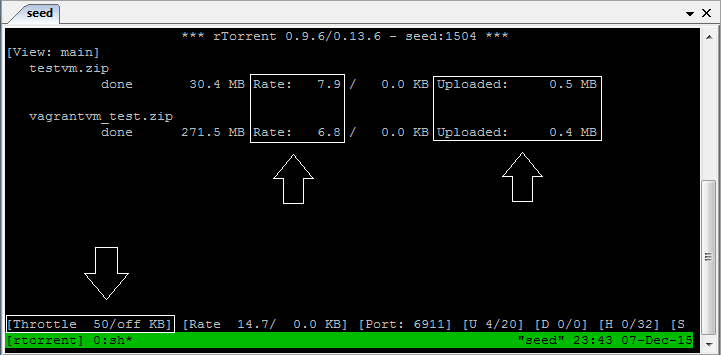
\includegraphics[width=120mm, keepaspectratio]{figures/test_seed_torrent.png}
\caption{Rtorrent: Futó feltöltések}
\label{fig:seed_torrent}
\end{figure}

A két futó fájlátvitel részleteit megnézve ellenőrizhetjük, hogy a megfelelő gépek töltenek-e le. Például a ``customvm\_test''-et tartalmazó testvm.zip-et a labpc101 és 103-nak kellene töltenie, lásd \ref{fig:seed_peers}-es~ábra (a két gép IP címe .111 ill. .113-ra végződik).

\begin{figure}[ht]
\centering
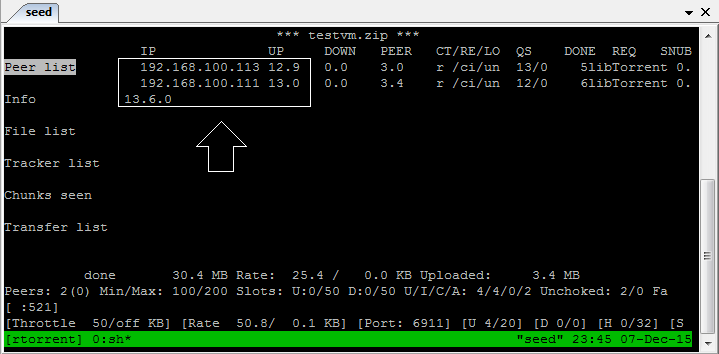
\includegraphics[width=120mm, keepaspectratio]{figures/test_seed_peers.png}
\caption{Rtorrent: Torrent részletei}
\label{fig:seed_peers}
\end{figure}

Egy pár percen belül véget is ér a terítés:\\\\
\code{2015-12-08 00:46:40 INFO hu.bme.mit.vmdistribution.app.distrstatus.DistributionStatusUpdater run [All transfers are finished, distribution is complete, press ENTER to continue.]}\\
\code{2015-12-08 00:46:57 INFO hu.bme.mit.vmdistribution.app.UseModel main [Saving changes to model instance.]}\\
\code{2015-12-08 00:46:57 INFO hu.bme.mit.vmdistribution.app.UseModel main [Done.]}\\\\

A modellünket tartalmazó fájlt közelebbről megnézve ellenőrizhetjük, hogy az tényleg frissült-e, a labpc101-et reprezentáló Computer objektum például most már így néz ki:\\\\
\code{<computers virtualmachines="//@virtualmachines.1 //@virtualmachines.0" name="labpc101" maxSpaceForVMs="40000.0" installedRAM="8000.0" architecture="x64">}\\\\
A Computer-en levő virtuális gépeket a virtualmachines lista tárolja, aminek a két eleme a terített virtuális gépek objektumaira mutat.\\

Befejeztük az alkalmazás tesztelését, az elvárt eredményre jutottunk.

%----------------------------------------------------------------------------
\section{Teljesítményelemzés}
%----------------------------------------------------------------------------
A programom teljesítményének elemzéséhez a következő méréseket végeztem el:

\begin{itemize}
  \item 1,2,4 és 8 GB méretű fájlok terítése 10 ill. 25 gépre
  \item 4 GB méretű fájl terítése 25 gépre háromszor, különböző seed választásával
  \item Hibatűrési tesztek a terítés elején hiányzó, ill. aközben kieső gépekkel.
\end{itemize}

Továbbá, hogy legyen összehasonlítási alap  az eredeti Chaincast alapú terítést is lefuttattam 25 gépre 1,2,4 és 8 GB méretű fájlokkal.
A mérési eredmények az alkalmazásom futásakor keletkező logfájlból származnak, Chaincast esetében pedig a Jenkins webes felületén a terítéshez tartozó build ``build output'' részből.

%
\subsection{Chaincast és Torrent alapú terítés idejének összehasonlítása}
%

Nem a gyorsabb fájlterítés megvalósítása volt a programom egyik célja, de attól még érdemes lehet összehasonlítanunk a két módszer sebességét, hiszen mindegy mennyit nyerünk a robusztusságon , ha használhatatlanul lassabb lesz az alkalmazás a mostaninál. Az~\ref{fig:chaincasttorrrentcomparison}-es~ábrán láthatjuk a különböző méretű fájlok terítésének az idejét. Előtte viszont érdemes részletesebben megnézni, hogy ez az idő konkrétan mit (nem) tartalmaz:

\begin{itemize}
  \item Egyik megoldásnál sem tartalmazza a terítés ideje a terítendő fájlok létrehozását, és a központi gépre másolását (ami egyik esetben egy hálózati meghajtó, másik esetben a torrent-es terítés seed-je)
  \item Torrent-es terítésnél az időt a fájl hash-elése előtt, illetve után kezdjük mérni, Chaincast-nál a webes felületen a terítés indításától
\end{itemize}

Az előbbi állítások a későbbi mérésekre is igazak lesznek.

\begin{figure}[ht]
\centering
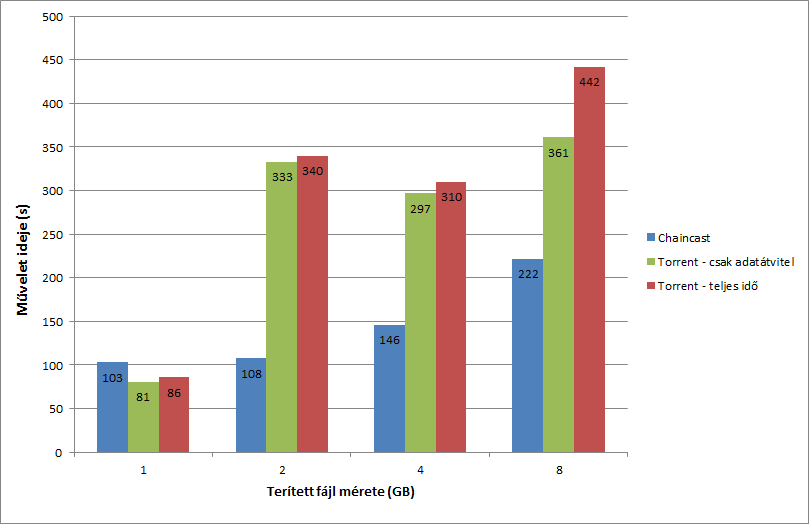
\includegraphics[width=150mm, keepaspectratio]{figures/Perf_chaincast_torrent_comparison.png}
\caption{Chaincast és Torrent alapú terítés idejének összehasonlítása}
\label{fig:chaincasttorrrentcomparison}
\end{figure}

Az eredményekből látszik, hogy sebesség terén elfogadható, amit kaptunk: nagyobb fájloknál körülbelül kétszer lassabb a terítés a Chaincast-hoz képest, és az a tapasztalat, hogy hogy átlagosan 2 próbálkozás kell egy sikeres Chaincast-os terítéshez, ami ha a vége felé szakadna meg a sikertelen próba során, akkor összességében hasonló időt venne igénybe. Kis fájloknál sokkal kevésbé jelentős a két módszer sebessége közti különbség, viszont az nem derült ki, hogy milyen anomália lépett fel a 2 GB-os fájl terítése során, hiszen az tovább tartott, mint a 4 GB-osé. Az is megjegyzendő, hogy a seed gépen a feltöltés indítása előtti hash-ellenőrzés okozta időveszteség (lásd a Torrent alapú terítéshez kapcsolódó oszloppárok közti különbség) nem lineárisan nő a feltöltendő fájl méretéhez képest, ezért nagyon javasolt lenne a torrentklienset rákényszeríteni ennek az ellenőrzésnek a kihagyására.

%
\subsection{Skálázódás - Torrent alapú terítés 10 és 25 gépere}
%

A Torrent-től, mint P2P alapú fájlmegosztó protokolltól azt várjuk, hogy letöltők számával minimum nem fordítottan arányos a terítés ideje, vagyis több résztvevő esetén sem tart több ideig a fájlátvitel. Most 10 és 25 gépre történő térítés esetén hasonlítjuk össze teljesítménymutatókat a következő táblázat segítségével:

\begin{center}
	\begin{tabular}{ |c|>{\centering\arraybackslash}m{2.5cm}|>{\centering\arraybackslash}m{2.5cm}|>{\centering\arraybackslash}m{2.5cm}|>{\centering\arraybackslash}m{2.5cm}| }
		\hline
		\multirow{2}{*}{Fájlméret}&\multicolumn{2}{|c|}{Terítés - teljes idő}&\multicolumn{2}{|c|}{Terítés - csak az adatátvitel} \\
		& 10 gépre & 25 gépre & 10 gépre & 25 gépre \\
		\hline
		1 GB & 85 s & 86 s & 80 s & 81 s \\
		\hline
		2 GB & 178 s & 340 s & 167 s & 333 s \\
		\hline
		4 GB & 293 s & 310 s & 270 s & 297 s \\
		\hline
		8 GB & 563 s & 442 s & 516 s & 361 s \\
		\hline
	\end{tabular}
\end{center}

[a szegélyeket hogyan lehetne szépre megcsinálni?]\\%TODO

Számunkra kedvező eredményt kaptunk, hiszen nagyobb fájlok terítésénél nemhogy lassabb lett 15 célgép hozzáadásával a terítés, hanem érezhetően gyorsabb. A Torrent protokoll működését ismerve lassulással nem is kellett volna számolnunk, hiszen ideális esetben a letöltés idejét kizárólag a seed feltöltési sebessége határozza meg. [ezt bővebben kifejteni a háttérismeretek Torrentes részében, vagy a tervezésnél és innen visszahivatkozni talán.]%TODO

%
\subsection{Terítés ideje különbőző seed-ek választása esetén}
%

Érdemes lehet megnézni, hogy más-más seed gép választása hogyan befolyásolja a terítés idejét, ezért lefuttattam a 4 GB-os fájl terítését 25 gépre háromszor, különböző seed-et választva. Az eredményt az~\ref{fig:differentseedscomparison}-es~ábra szemlélteti. 

\begin{figure}[ht]
\centering
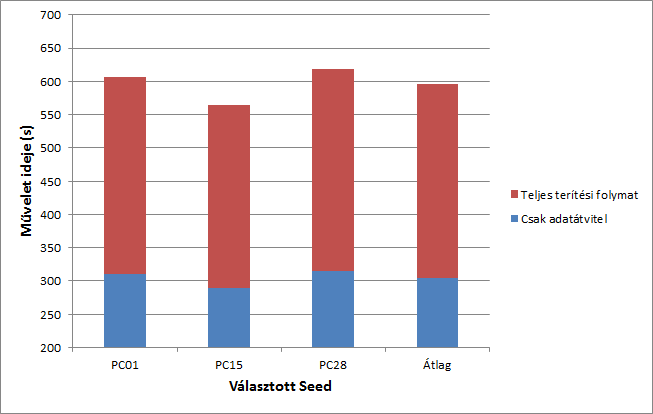
\includegraphics[width=120mm, keepaspectratio]{figures/Perf_different_seeds.png}
\caption{Terítés ideje különbőző seed-ek választása esetén}
\label{fig:differentseedscomparison}
\end{figure}

Látható, hogy különösebben nincs jelentősége, hogy melyik gépet választjuk seed-nek, persze ha egy nem ennyire homogén gépparkkal felszerelt laborban végeztük volna a tesztelést, akkor feltétlen a leggyorsabb gépet kellett volna e feladatra választanunk.

%
\subsection{P2P alapú fájlterítés - hibatűrés}
%

A hibatűrési tesztet két részben végeztem el, az első részben azt néztem meg, hogy az én megoldásom hogyan reagál, ha a terítés indításakor van nem elérhető célgép. Ez Chaincast esetében automatikus bukást okoz, mivel ott küldés előtt ellenőrződik a teljes lánc létrejötte, és hiányzó gép esetében el sem kezdődik a fájlátvitel (pedig elvileg a lánc utolsó n db. gépének hiányával toleráns lehetne).\\
Az első teszthez 10 gépes terítést kíséreltem meg, úgy hogy a ``labpc03'' nevezetű kikapcsolt állapotban volt, a futást kövessük nyomon a program kimenetében:\\\\
Minden rendben történik egészen addig a lépésig, amíg a terítendő fájlhoz tartozó torrentfájlt nem próbáljuk labpc03-ra másolni:\\\\
\code{2015-12-05 10:37:57 INFO hu.bme.mit.vmdistribution.app.vmutil.TorrentUtil copyTorrentFile [Copying torrent file test\_1g.torrent to labpc03.]}\\
\code{2015-12-05 10:38:01 SEVERE hu.bme.mit.vmdistribution.app.ssh.SSHUtil remoteExec ssh: connect to host 10.40.2.31 port 22: No route to host}\\\\
Azt a nem meglepő eredmény kaptuk, hogy nem sikerült a másolás, de ettől független a többi gépre igen, például a labpc08-ra(akinek az IP címe 10.40.2.140):\\\\
\code{2015-12-05 10:37:57 INFO hu.bme.mit.vmdistribution.app.ssh.SSHUtil remoteExec Copied test\_1g.torrent to 10.40.2.140:\textasciitilde/Torrents}\\\\
A torrent fájlok sikeres felmásolásával és a torrent kliensek elindításával elkezdődnek a letöltések, amelyeknek állapotáról 10 másodpercenként kapunk információkat. Ehhez hasonló üzeneteket fogunk látni:\\\\
\code{2015-12-05 10:43:51 INFO hu.bme.mit.vmdistribution.app.distrstatus.DistributionStatusUpdater run 	labpc08:}\\
\code{2015-12-05 10:43:51 INFO hu.bme.mit.vmdistribution.app.distrstatus.DistributionStatusUpdater run 		[ test\_1g: Completed: 13\%, Downloaded: 141.03/1024.0 MB, Speed: 2.35 MB/s.}\\\\
Persze csak a hiányzó gép okozta hibaüzenetek mellett:\\\\
\code{2015-12-05 10:43:54 SEVERE hu.bme.mit.vmdistribution.app.distrstatus.RTorrentXmlRpcClient updateTransferStatus ERROR executing XMLRPC call.
org.apache.xmlrpc.XmlRpcException: Failed to read server's response: No route to host}\\\\
A bekapcsolva hagyott gépekre végül eljut a terítendő fájl és a program futását manuálisan megszakítjuk:\\\\
\code{2015-12-05 10:45:59 INFO hu.bme.mit.vmdistribution.app.UseModel distributionProgressLoop Quit due to user command}\\
\code{2015-12-05 10:45:59 WARNING hu.bme.mit.vmdistribution.app.UseModel distributionProgressLoop [There were unfinished transfers:]}\\
\code{2015-12-05 10:45:59 WARNING hu.bme.mit.vmdistribution.app.UseModel distributionProgressLoop test\_1g->labpc03 }\\\\
A második teszt folyamán a fájlátvitel közben tettem gépeket elérhetetlenné, ennél a mérésnél a ``labpc06'' és ``labpc08'' nevű gépeken adatátvitel közben bezártam a torrentklienseket, illetve a ``labpc10''-nek szűntettem meg a hálózati csatlakozását. Miután a többi gépre sikeresen eljutott a terítendő fájl a három kieső gépet ``helyreállítottam'', ezek után behozták a lemaradást és befejezték a letöltést, így végül sikerrel zárult folyamat:\\\\
\code{2015-12-05 10:56:09 INFO hu.bme.mit.vmdistribution.app.distrstatus.DistributionStatusUpdater run [All transfers are finished, distribution is complete, press ENTER to continue.]}

%
\subsection{P2P alapú fájlterítés - szűk keresztmetszetek}
%

A többi mérés elvégzése közben feltűnt, hogy sokszor ugyanazok a gépek fejezték be utoljára a letöltést, úgyhogy összegyűjtöttem a~\ref{fig:computerdownloadspeeds}-es ábrán látható diagramokon, hogy adott gép hányszor szerepelt a terítések végén a 3 leglassabb, illetve leggyorsabb gép között:


\begin{figure}[ht]
\centering
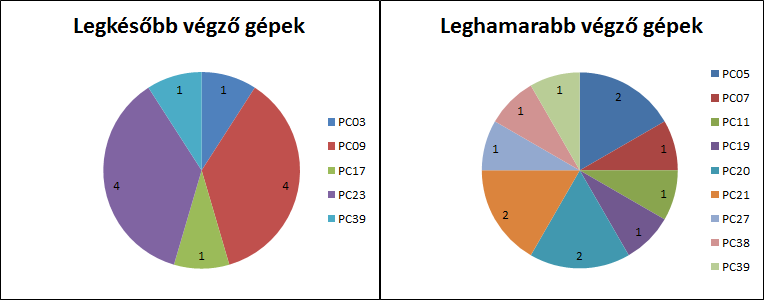
\includegraphics[width=150mm, keepaspectratio]{figures/Perf_computers.png}
\caption{Letöltést leghamarabb/legkésőbb befejező gépek}
\label{fig:computerdownloadspeeds}
\end{figure}

Mindkét esetben azt kellene látnunk, hogy a gépek alacsony gyakorisággal és véletlenül szerepelnek a toplistáinkon, viszont a leglassabb gépek között 23 és 9 sorszámúak kirívóan nagy gyakoriságot értek el, feltehetőleg a gépek hálózati kapcsolatával, vagy magukkal a gépekkel kapcsolatban vannak kijavítandó problémák, őket ezek megoldásáig nem érdemes seed-nek választani.

%
%\subsection{P2P alapú fájlterítés - letöltési sebességek}
%
%ha nagyon kell még oldalszám miatt extra, akkor jöhet, de amúgy elég szegényes ez a mérés 
%TODO

